% Ghi chú: Nội dung đặc tả phân hệ Văn bản đến đã được tích hợp và chuẩn hoá vào 
% Chapter4/section2/ioffice_schedule/index.tex (gồm FR-IOFF và UC-OFF-01 -> UC-OFF-04)
% để đảm bảo tính nhất quán với cấu trúc 4 nhóm phân hệ của báo cáo (Bảng 4.1 và Chương 5).
% File này được giữ lại làm tài liệu tham khảo chi tiết.

\subsection{Phân hệ quản lý văn bản đến}
\label{subsec:incoming_docs}

\subsubsection{Mục tiêu}
Trong hoạt động quản trị đại học về công tác tiếp nhận, xử lý, phân công và lưu trữ văn bản đến (công văn, chỉ thị, tờ trình, thông báo, quyết định từ Bộ Giáo dục và Đào tạo, các cơ quan ban ngành và đối tác bên ngoài) là một trong những mạch thông tin và điều hành trọng yếu nhất. Trước khi ứng dụng giải pháp số hóa, quy trình xử lý văn bản giấy truyền thống tồn tại nhiều bất cập: thời gian luân chuyển hồ sơ vật lý chậm trễ qua nhiều cấp (Văn thư $\rightarrow$ Lãnh đạo Phòng Hành chính $\rightarrow$ Ban Giám hiệu $\rightarrow$ Lãnh đạo các đơn vị, ...) gây khó khăn trong việc giám sát tiến độ thực tế dẫn đến tình trạng tồn đọng hoặc quá hạn xử lý không được cảnh báo kịp thời; rủi ro thất lạc, hư hỏng tài liệu quan trọng trong quá trình sao chụp.

Phân hệ Quản lý văn bản đến nhằm số hóa toàn diện quy trình tiếp nhận, luân chuyển, phê duyệt, phân công và giám sát văn bản trong toàn trường trên môi trường mạng. Quy trình nghiệp vụ điện tử được chuẩn hóa xuyên suốt qua 4 bước: Tiếp nhận \& Tham mưu $\rightarrow$ Trình \& Chỉ đạo $\rightarrow$ Triển khai các đơn vị $\rightarrow$ Hoàn thành.

\subsubsection{Yêu cầu chức năng}
\begin{itemize}
    \item \textbf{FR-ID-01 -- Tiếp nhận và đăng ký văn bản đến:} Văn thư tiếp nhận hồ sơ văn bản bên ngoài, soạn thảo các thông tin văn bản để hệ thống tự động kích hoạt cấu hình quy trình mẫu tương ứng, tạo hồ sơ văn bản điện tử và tự động phân quyền xem bước đầu cho nhân sự phụ trách.
    \item \textbf{FR-ID-02 -- Cấp số đến tự động từ quỹ số:} Hệ thống tự động sinh số đến tăng dần duy nhất trong năm hành chính từ Quỹ số tập trung; hỗ trợ kiểm tra tính duy nhất chống trùng lặp; tự động giải phóng và thu hồi số đến khi hồ sơ văn bản bị xóa.
    \item \textbf{FR-ID-03 -- Quản lý tệp đính kèm:} Hỗ trợ tải lên đa tệp tài liệu số hóa (PDF, Word, hình ảnh: \texttt{.pdf}, \texttt{.docx}, \texttt{.png}, \texttt{.jpg}...), tự động mã hóa tên tệp và lưu trữ an toàn.
    \item \textbf{FR-ID-04 -- Tham mưu đề xuất xử lý văn bản:} Lãnh đạo và Văn thư Phòng Hành chính tiến hành tổng hợp nghiên cứu nội dung văn bản, ghi nhận ý kiến tham mưu đề xuất xử lý, lập dự thảo phương án phân công đến các đơn vị/cá nhân.
    \item \textbf{FR-ID-05 -- Ban Giám hiệu chỉ đạo điều hành:} Ban Giám hiệu xem xét hồ sơ văn bản, tệp đính kèm và ý kiến tham mưu; ghi ý kiến chỉ đạo điều hành, phê duyệt phương án phân công.
    \item \textbf{FR-ID-06 -- Phân công trách nhiệm linh hoạt:} Thiết lập các dòng phân công gắn với đơn vị hoặc đích danh cá nhân theo 6 vai trò nghiệp vụ xác định: \textit{Chỉ đạo thực hiện, Đồng chỉ đạo (chỉ dành cho BGH), Thực hiện chính, Phối hợp thực hiện, Trả lời và Nhận để biết}.
    \item \textbf{FR-ID-07 -- Cơ chế đồng thuận đa chỉ đạo:} Khi phân công có nhiều lãnh đạo đồng chỉ đạo, văn bản chỉ được chuyển tiếp khi tất cả các lãnh đạo đồng chỉ đạo đã hoàn tất ghi nhận ý kiến chỉ đạo.
    \item \textbf{FR-ID-08 -- Tiếp nhận văn bản tại đơn vị/cá nhân thụ lý:} Lãnh đạo hoặc chuyên viên đơn vị thực hiện xác nhận tiếp nhận văn bản.
    \item \textbf{FR-ID-09 -- Hỗ trợ tra cứu, lọc và giám sát tiến độ:} Hỗ trợ phân loại và lọc văn bản, cho phép xem chi tiết dòng thời gian tiến trình luân chuyển và bảng tiến độ thực hiện của từng đơn vị.
\end{itemize}

\subsubsection{Đặc tả usecase}
\begin{figure}[H]
    \centering
    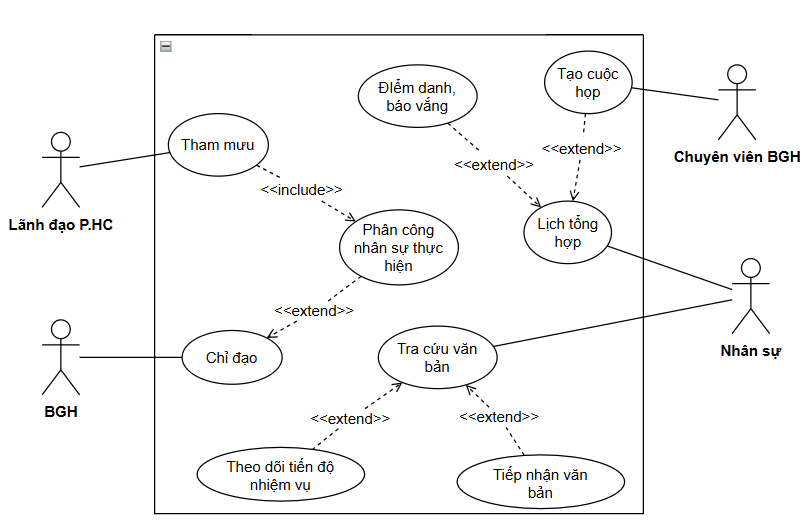
\includegraphics[width=\linewidth]{image/usecase/UC_DOC.png}
    \caption{Sơ đồ use\-case quản lý văn bản đến}
    \label{fig:DOC_UC}
\end{figure}

\usecasespec{
    id={UC\_DOC\_01},
    name={Tiếp nhận và Đăng ký Văn bản đến mới},
    actor={Văn thư trường (Phòng Hành chính -- Tổng hợp)},
    desc={Tiếp nhận văn bản từ bên ngoài, tạo hồ sơ văn bản điện tử, hệ thống tự động cấp số đến duy nhất từ Quỹ số và khởi tạo các bước quy trình luân chuyển.},
    pre={Người dùng đăng nhập với vai trò Văn thư trường; Quỹ số văn bản đến của năm hiện tại đang được kích hoạt (\texttt{apDung = 1}).},
    trigger={Văn thư truy cập trang Quản lý Văn bản đến và nhấn nút "Tạo mới".},
    mainflow={
            1. Hệ thống hiển thị danh mục các Loại văn bản được cấu hình quy trình mẫu. \newline
            2. Văn thư chọn loại văn bản tương ứng và gửi yêu cầu khởi tạo. \newline
            3. Hệ thống mở giao dịch CSDL: kiểm tra Quỹ số năm hiện tại và tự động sinh số đến tiếp theo duy nhất. \newline
            4. Hệ thống tạo bản ghi văn bản đến, ghi nhận số đến vào \texttt{eoffice\_van\_ban\_den\_so\_den}. \newline
            5. Hệ thống đọc cấu hình quy trình mẫu và sinh các bước xử lý tương ứng vào \texttt{eoffice\_van\_ban\_den\_quy\_trinh}. \newline
            6. Hệ thống cập nhật trạng thái văn bản sang bước đầu tiên (\texttt{leaderAdvisory}) và cấp quyền truy cập ban đầu cho người tạo và nhân sự bước 1. \newline
            7. Hệ thống commit giao dịch và chuyển sang giao diện chi tiết để tiếp tục hoàn thiện hồ sơ.
        },
    altflow={
            3.1. Quỹ số của năm hiện tại chưa được kích hoạt hoặc hết số: Hệ thống rollback giao dịch, hiển thị thông báo lỗi và yêu cầu quản trị viên cấu hình Quỹ số mới. \newline
            5.1. Loại văn bản chưa được gắn cấu hình quy trình mẫu: Hệ thống hủy giao dịch và cảnh báo chưa có quy trình áp dụng.
        },
    post={Hồ sơ văn bản đến được tạo lập thành công; số đến được cấp phát duy nhất và danh sách các bước quy trình được khởi tạo đầy đủ.},
    label={tab:uc_doc_01}
}

\usecasespec{
    id={UC\_DOC\_02},
    name={Cập nhật Thông tin văn bản và Quản lý Tệp đính kèm},
    actor={Văn thư trường, Cán bộ có quyền chỉnh sửa văn bản},
    desc={Cập nhật các thuộc tính hành chính của hồ sơ văn bản và tải lên, quản lý các tệp tài liệu số hóa kèm theo văn bản.},
    pre={Văn bản đã tồn tại trên hệ thống và người dùng có quyền \texttt{canModifyDocument} tại bước hiện tại.},
    trigger={Người dùng mở màn hình chi tiết văn bản và thực hiện chỉnh sửa hoặc tải tệp.},
    mainflow={
            1. Người dùng cập nhật các trường hành chính: Trích yếu, Số/ký hiệu văn bản, Đơn vị gửi, Ngày văn bản, Hạn hoàn thành, Ghi chú, Tính chất khẩn. \newline
            2. Người dùng chọn một hoặc nhiều tệp đính kèm (scan, phụ lục) và tải lên hệ thống. \newline
            3. Hệ thống kiểm tra tính hợp lệ của tệp, đổi tên sang định danh ngẫu nhiên và lưu trữ an toàn trong phân vùng tài nguyên. \newline
            4. Hệ thống ghi nhận thông tin tệp vào bảng quản lý tệp (\texttt{fwFile}) và liên kết với văn bản (\texttt{eoffice\_van\_ban\_den\_file}). \newline
            5. Người dùng nhấn nút "Lưu thay đổi". \newline
            6. Hệ thống cập nhật dữ liệu văn bản; nếu văn bản đã liên kết nhiệm vụ, hệ thống tự động đồng bộ lại thời hạn hoàn thành (\texttt{endDate}) của nhiệm vụ. \newline
            7. Hệ thống thông báo cập nhật thành công và ghi nhận nhật ký thao tác.
        },
    altflow={
            1.1. Văn bản đã ở trạng thái Hoàn thành (\texttt{departmentsDone}): Hệ thống khóa các trường số văn bản và độ khẩn, chỉ cho phép chỉnh sửa trích yếu, ghi chú và phân loại thông tin. \newline
            2.1. Người dùng chọn xóa tệp đính kèm: Hệ thống thực hiện xóa mềm bản ghi liên kết và ghi nhật ký kiểm toán.
        },
    exflow={
            3.1. Tệp đính kèm vượt quá dung lượng cho phép hoặc sai định dạng: Hệ thống báo lỗi, dọn dẹp tệp tạm và giữ nguyên trạng thái cũ.
        },
    post={Thông tin hành chính của văn bản và danh sách tệp đính kèm được lưu trữ an toàn; thời hạn nhiệm vụ liên kết được đồng bộ.},
    label={tab:uc_doc_02}
}

\usecasespec{
    id={UC\_DOC\_03},
    name={Tham mưu Xử lý Văn bản đến},
    actor={Lãnh đạo Phòng Hành chính -- Tổng hợp, Văn thư trường},
    desc={Nghiên cứu nội dung văn bản, ghi ý kiến tham mưu đề xuất xử lý, lập dự thảo phân công trên Phiếu Giải Quyết và chuyển tiếp hồ sơ trình Ban Giám hiệu.},
    pre={Văn bản đang ở trạng thái \texttt{received} hoặc \texttt{leaderAdvisory}; người dùng có quyền \texttt{canThamMuu = true}.},
    trigger={Lãnh đạo hoặc Văn thư mở văn bản trong tab "Chờ tham mưu" hoặc "Chờ xử lý".},
    mainflow={
            1. Người dùng xem toàn văn tệp đính kèm và thông tin trích yếu văn bản. \newline
            2. Người dùng nhập nội dung ý kiến tham mưu đề xuất vào ô ý kiến xử lý. \newline
            3. Người dùng lập dự thảo danh sách phân công đơn vị/cá nhân trên Phiếu Giải Quyết (chọn đơn vị chủ trì, phối hợp, để biết). \newline
            4. Người dùng nhấn nút "Trình Ban Giám hiệu" (hoặc "Chuyển tiếp"). \newline
            5. Hệ thống kiểm tra nếu chưa có hạn hoàn thành, tự động gán hạn mặc định bằng ngày nhận cộng 7 ngày. \newline
            6. Hệ thống ghi nhận ý kiến tham mưu, thời gian và thông tin người thực hiện vào bảng lịch sử quy trình (\texttt{eoffice\_van\_ban\_den\_quy\_trinh\_history}). \newline
            7. Hệ thống nâng trạng thái văn bản sang bước Chờ chỉ đạo (\texttt{directorCommand}) và tự động cấp quyền truy cập cho Ban Giám hiệu. \newline
            8. Hệ thống phát sự kiện thông báo thời gian thực qua Socket.IO đến Ban Giám hiệu.
        },
    exflow={
            4.1. Hồ sơ chưa có số văn bản hoặc chưa đính kèm tệp tài liệu: Hệ thống cảnh báo thiếu điều kiện chuyển bước và yêu cầu bổ sung trước khi trình.
        },
    post={Ý kiến tham mưu được ghi nhận vào lịch sử luân chuyển; văn bản chuyển sang trạng thái \texttt{directorCommand}; Ban Giám hiệu nhận thông báo xử lý.},
    label={tab:uc_doc_03}
}

\usecasespec{
    id={UC\_DOC\_04},
    name={Ban Giám hiệu Chỉ đạo và Phê duyệt Phân công},
    actor={Hiệu trưởng, Phó Hiệu trưởng (Ban Giám hiệu)},
    desc={Ban Giám hiệu xem xét ý kiến tham mưu, đưa ra ý kiến chỉ đạo điều hành, phê duyệt phương án phân công trên Phiếu Giải Quyết và kích hoạt triển khai văn bản.},
    pre={Văn bản đang ở trạng thái \texttt{directorCommand}; người dùng thuộc Ban Giám hiệu và có quyền \texttt{canChiDao = true}.},
    trigger={Lãnh đạo BGH mở văn bản trong tab "Chờ chỉ đạo".},
    mainflow={
            1. Lãnh đạo BGH xem xét nội dung tệp đính kèm, trích yếu và ý kiến tham mưu của Phòng Hành chính. \newline
            2. Lãnh đạo nhập nội dung chỉ đạo điều hành vào ô ý kiến chỉ đạo. \newline
            3. Lãnh đạo xem xét, điều chỉnh hoặc xác nhận danh sách phân công trên Phiếu Giải Quyết (PGQ). \newline
            4. Lãnh đạo nhấn nút "Chỉ đạo \& Triển khai" (hoặc "Lưu chỉ đạo"). \newline
            5. Hệ thống thiết lập khóa giao dịch cơ sở dữ liệu (\texttt{SELECT pg\_advisory\_xact\_lock(1001, :id)}) để ngăn ngừa xung đột dữ liệu. \newline
            6. Hệ thống lưu ý kiến chỉ đạo vào lịch sử quy trình và đồng bộ nội dung vào hộp thảo luận chung (\texttt{commentGeneral}). \newline
            7. Hệ thống kiểm tra điều kiện triển khai: Người chỉ đạo chính và tất cả các Người đồng chỉ đạo đã hoàn tất ghi nhận ý kiến chỉ đạo. \newline
            8. Nếu đủ điều kiện triển khai: Hệ thống chuyển trạng thái văn bản sang Đã triển khai (\texttt{sentToDepartments}) và ghi nhận thời điểm \texttt{deploymentAt}. \newline
            9. Nếu văn bản không phải là loại thuần thông tin: Hệ thống tự động kích hoạt tạo cây Nhiệm vụ liên phòng ban (Parent Task và Subtasks) bên phân hệ Nhiệm vụ. \newline
            10. Hệ thống tự động cấp quyền truy cập văn bản cho Ban chủ nhiệm và Văn thư các đơn vị được phân công trong PGQ, commit giao dịch và giải phóng khóa.
        },
    altflow={
            7.1. Còn thành viên Ban Giám hiệu đồng chỉ đạo chưa cho ý kiến: Hệ thống lưu lại ý kiến của lãnh đạo hiện tại, giữ nguyên trạng thái văn bản ở \texttt{directorCommand} để chờ các lãnh đạo còn lại hoàn tất chỉ đạo.
        },
    post={Ý kiến chỉ đạo được ghi nhận; văn bản chuyển sang trạng thái \texttt{sentToDepartments} khi đủ đồng thuận; nhiệm vụ liên phòng ban được tạo tự động.},
    label={tab:uc_doc_04}
}

\usecasespec{
    id={UC\_DOC\_05},
    name={Lập và Điều chỉnh Phiếu Giải Quyết (PGQ)},
    actor={Lãnh đạo/Văn thư Phòng Hành chính (dự thảo), Ban Giám hiệu (phê duyệt)},
    desc={Thiết lập, cập nhật hoặc xóa các dòng phân công trách nhiệm cho các đơn vị hoặc cá nhân thụ lý gắn liền với hồ sơ văn bản đến.},
    pre={Người dùng có thẩm quyền lập hoặc chỉnh sửa Phiếu Giải Quyết (\texttt{canEditPhieuGiaiQuyet = true}).},
    trigger={Người dùng mở panel Phiếu Giải Quyết trên màn hình chi tiết văn bản.},
    mainflow={
            1. Người dùng chọn thao tác thêm mới một dòng phân công trên PGQ. \newline
            2. Người dùng lựa chọn đơn vị thụ lý (từ danh mục phòng ban) hoặc chỉ định đích danh cán bộ (qua mã số cán bộ \texttt{shcc}). \newline
            3. Người dùng tích chọn vai trò trách nhiệm: Chỉ đạo thực hiện, Đồng chỉ đạo, Thực hiện chính, Phối hợp thực hiện, Trả lời hoặc Để biết. \newline
            4. Hệ thống kiểm tra ràng buộc: vai trò chỉ đạo và đồng chỉ đạo bắt buộc phải thuộc đơn vị Ban Giám hiệu (đơn vị \texttt{01} hoặc \texttt{14}). \newline
            5. Hệ thống lưu bản ghi vào \texttt{eoffice\_van\_ban\_den\_phieu\_giai\_quyet} và tự động bổ sung quyền xem văn bản vào \texttt{eoffice\_van\_ban\_den\_user}. \newline
            6. Nếu văn bản đã ở trạng thái \texttt{sentToDepartments}, hệ thống tự động phát sự kiện Message Queue để sinh thêm Subtask tương ứng bên hệ thống Nhiệm vụ. \newline
            7. Hệ thống ghi nhật ký kiểm toán thao tác phân công vào \texttt{eoffice\_van\_ban\_den\_log}.
        },
    altflow={
            1.1. Người dùng sửa đổi vai trò của dòng PGQ đã tạo: Hệ thống cập nhật bản ghi và điều chỉnh lại quyền hạn tương ứng. \newline
            1.2. Người dùng xóa một dòng phân công: Hệ thống thu hồi quyền xem văn bản của nhân sự đó và xóa Subtask tương ứng bên hệ thống Nhiệm vụ.
        },
    exflow={
            1.3. Cố gắng xóa dòng PGQ đã được tiếp nhận (\texttt{receivedAt != null}) hoặc đã hoàn thành (\texttt{doneAt != null}): Hệ thống từ chối thao tác và cảnh báo vi phạm tính toàn vẹn dữ liệu.
        },
    post={Danh sách phân công PGQ được cập nhật chính xác; quyền truy cập và các nhiệm vụ liên kết được đồng bộ tức thời.},
    label={tab:uc_doc_05}
}

\usecasespec{
    id={UC\_DOC\_06},
    name={Tiếp nhận Văn bản tại Đơn vị / Cá nhân},
    actor={Lãnh đạo Đơn vị, Văn thư Đơn vị, Chuyên viên thụ lý},
    desc={Đơn vị hoặc cá nhân được phân công trên Phiếu Giải Quyết thực hiện thao tác xác nhận tiếp nhận văn bản để bắt đầu xử lý công việc.},
    pre={Văn bản đang ở trạng thái \texttt{sentToDepartments}; người dùng thuộc đơn vị hoặc là cá nhân có dòng PGQ chưa tiếp nhận (\texttt{receivedAt == null}).},
    trigger={Người dùng mở văn bản từ danh sách "Chờ xử lý" và bấm nút "Tiếp nhận".},
    mainflow={
            1. Người dùng xem thông tin trích yếu, tệp đính kèm và ý kiến chỉ đạo của Ban Giám hiệu. \newline
            2. Người dùng nhấn nút "Tiếp nhận" văn bản. \newline
            3. Hệ thống mở giao dịch CSDL: ghi nhận thời điểm tiếp nhận (\texttt{receivedAt}) và định danh người tiếp nhận (\texttt{receivedBy}) vào dòng PGQ. \newline
            4. Hệ thống ghi nhận sự kiện vào lịch sử quy trình luân chuyển (\texttt{eoffice\_van\_ban\_den\_quy\_trinh\_history}). \newline
            5. Nếu văn bản có liên kết nhiệm vụ: Hệ thống tự động cập nhật người dùng vào danh sách tham gia nhiệm vụ (\texttt{missionParticipant.joinMission}). \newline
            6. Hệ thống kiểm tra tính chất văn bản: Nếu là văn bản thuần thông tin (\texttt{isThongTin = true}) hoặc vai trò phân công là Để biết (\texttt{biet = true}), hệ thống tự động gán luôn \texttt{doneAt = receivedAt} và \texttt{doneBy = receivedBy}. \newline
            7. Hệ thống kiểm tra nếu toàn bộ các dòng PGQ thực hiện đã hoàn tất, tự động nâng trạng thái văn bản lên \texttt{departmentsDone}. \newline
            8. Commit giao dịch, gửi thông báo cập nhật và phản hồi thành công cho người dùng.
        },
    post={Dòng PGQ được ghi nhận trạng thái đã tiếp nhận; người dùng được tham gia vào nhiệm vụ liên kết; văn bản thông tin được tự động hoàn tất.},
    label={tab:uc_doc_06}
}

\usecasespec{
    id={UC\_DOC\_07},
    name={Báo cáo Hoàn thành Xử lý Văn bản đến},
    actor={Lãnh đạo Đơn vị, Chuyên viên thụ lý (vai trò Thực hiện chính hoặc Phối hợp)},
    desc={Sau khi hoàn thành phần việc được giao theo chỉ đạo của văn bản, đơn vị hoặc cá nhân báo cáo kết thúc xử lý trên hệ thống.},
    pre={Văn bản đang ở trạng thái \texttt{sentToDepartments}; dòng PGQ đã được tiếp nhận (\texttt{receivedAt != null}) và chưa hoàn thành (\texttt{doneAt == null}).},
    trigger={Người dùng mở văn bản và nhấn nút "Hoàn thành" trên giao diện chi tiết.},
    mainflow={
            1. Người dùng kiểm tra kết quả xử lý công việc và nhập ghi chú kết quả giải quyết (nếu có). \newline
            2. Người dùng nhấn nút "Hoàn thành". \newline
            3. Hệ thống cập nhật thời điểm hoàn thành (\texttt{doneAt}) và người báo cáo (\texttt{doneBy}) cho dòng PGQ tương ứng. \newline
            4. Hệ thống ghi nhận bản ghi hoàn tất vào lịch sử quy trình luân chuyển. \newline
            5. Hệ thống phát thông điệp Message Queue (\texttt{done-pgq:eoffice\_van\_ban\_den}) để tự động đóng Subtask tương ứng bên phân hệ Nhiệm vụ. \newline
            6. Hệ thống kiểm tra toàn bộ các dòng phân công thực hiện trong PGQ (ngoại trừ các dòng của Ban Giám hiệu). \newline
            7. Nếu 100\% các dòng thực hiện chính và phối hợp đều đã hoàn thành: Hệ thống tự động chuyển trạng thái văn bản sang Hoàn thành (\texttt{departmentsDone}). \newline
            8. Hệ thống phát sự kiện Socket.IO để cập nhật số liệu Dashboard và phản hồi kết quả thành công.
        },
    altflow={
            6.1. Vẫn còn đơn vị phối hợp hoặc thực hiện chính khác chưa hoàn thành: Hệ thống ghi nhận kết quả của đơn vị hiện tại và giữ nguyên trạng thái văn bản ở \texttt{sentToDepartments}.
        },
    post={Dòng PGQ ghi nhận trạng thái hoàn thành; nhiệm vụ liên kết được đóng; văn bản tự động chuyển sang \texttt{departmentsDone} khi toàn bộ các đơn vị xong việc.},
    label={tab:uc_doc_07}
}

\usecasespec{
    id={UC\_DOC\_08},
    name={Khởi tạo Văn bản đi Phúc đáp từ Văn bản đến},
    actor={Cán bộ thuộc đơn vị có vai trò Trả lời (\texttt{traLoi = true})},
    desc={Khởi tạo một dự thảo Văn bản đi mới liên kết trực tiếp với hồ sơ văn bản đến nhằm thực hiện nhiệm vụ trả lời hoặc phúc đáp cơ quan gửi văn bản.},
    pre={Văn bản đến đang xử lý hoặc đã hoàn thành; đơn vị của người dùng được phân công vai trò \texttt{traLoi = true} trên Phiếu Giải Quyết.},
    trigger={Người dùng nhấn nút chức năng "Tạo văn bản đi" trên màn hình chi tiết văn bản đến.},
    mainflow={
            1. Người dùng mở chi tiết văn bản đến, hệ thống hiển thị nút hành động "Tạo văn bản đi" (\texttt{canCreateVanBanDi = true}). \newline
            2. Người dùng nhấn nút "Tạo văn bản đi". \newline
            3. Hệ thống điều hướng người dùng sang biểu mẫu tạo lập dự thảo Văn bản đi của phân hệ \texttt{eoffice-van-ban-di}. \newline
            4. Hệ thống tự động kế thừa các thông tin: trích yếu nội dung (dạng "Phúc đáp cho văn bản đến số..."), nơi nhận (kế thừa từ đơn vị gửi của văn bản đến). \newline
            5. Người dùng hoàn thiện nội dung dự thảo Văn bản đi và lưu văn bản. \newline
            6. Hệ thống tự động ghi nhận mối quan hệ liên kết hai chiều vào bảng \texttt{eoffice\_van\_ban\_den\_van\_ban\_di\_relation}. \newline
            7. Người dùng có thể theo dõi tiến độ ban hành văn bản đi phúc đáp ngay trên dòng thông tin của văn bản đến gốc.
        },
    post={Dự thảo Văn bản đi được khởi tạo thành công; liên kết nguồn được lưu trữ chặt chẽ giữa hai phân hệ Văn bản đến và Văn bản đi.},
    label={tab:uc_doc_08}
}

\usecasespec{
    id={UC\_DOC\_09},
    name={Tra cứu, Lọc và Giám sát Tiến độ Văn bản đến},
    actor={Toàn thể cán bộ, giảng viên có quyền truy cập module (\texttt{eofficeVanBanDen:read})},
    desc={Tra cứu danh sách văn bản theo các tab nghiệp vụ, tìm kiếm theo tiêu chí hành chính, theo dõi dòng thời gian tiến trình và tiến độ xử lý của từng đơn vị.},
    pre={Người dùng đã đăng nhập vào hệ thống iOffice hoặc ứng dụng MyHCMUT Mobile.},
    trigger={Người dùng truy cập vào mục "Văn bản đến" từ menu chính.},
    mainflow={
            1. Người dùng chọn tab nghiệp vụ mong muốn: "Chờ xử lý", "Chờ tham mưu", "Chờ chỉ đạo", "Quá hạn", hoặc "Tất cả". \newline
            2. Người dùng nhập các tiêu chí tìm kiếm nâng cao: từ khóa trích yếu, số/ký hiệu văn bản, khoảng thời gian nhận, cơ quan gửi văn bản. \newline
            3. Hệ thống kiểm tra vai trò và phạm vi quyền truy cập của người dùng (\texttt{roleKey}, \texttt{maDonVi}, \texttt{shcc}). \newline
            4. Hệ thống truy vấn CSDL và trả về danh sách văn bản phân trang kèm theo trạng thái và thời hạn xử lý. \newline
            5. Người dùng chọn một văn bản cụ thể để xem chi tiết: \newline
            -- Xem thông tin hành chính, mức độ khẩn và thời hạn hoàn tất. \newline
            -- Xem và tải về các tệp đính kèm số hóa. \newline
            -- Xem dòng thời gian (Timeline) các bước đã chuyển tiếp kèm ý kiến tham mưu, chỉ đạo. \newline
            -- Xem tiến độ thực hiện chi tiết của từng đơn vị trên bảng Phiếu Giải Quyết (trạng thái tiếp nhận, hoàn thành). \newline
            -- Xem cây Nhiệm vụ liên kết và Văn bản đi phúc đáp (nếu có).
        },
    post={Người dùng nắm bắt toàn diện thông tin văn bản và tiến độ xử lý thực tế mà không làm thay đổi trạng thái dữ liệu gốc.},
    label={tab:uc_doc_09}
}

\subsubsection{Quy tắc nghiệp vụ}
\begin{itemize}
    \item \textbf{BR-DOC-01:} Số đến (\texttt{soDen}) là một số nguyên dương tăng dần liên tục và bắt buộc phải là duy nhất trong phạm vi một Quỹ số (\texttt{quySoId}) và một Năm hành chính (\texttt{nam}). Hệ thống nghiêm cấm việc nhập tay số đến; số đến phải được sinh tự động thông qua hàm quản lý quỹ số tập trung tại thời điểm tạo văn bản. Khi hồ sơ văn bản bị xóa ở bước khởi tạo ban đầu (\texttt{stepNo $\le$ 1}), bản ghi số đến tương ứng trong bảng \texttt{eoffice\_van\_ban\_den\_so\_den} sẽ bị giải phóng hoặc thu hồi để phục vụ mục đích kiểm toán sổ văn thư. Quỹ số được quản lý độc lập theo từng năm dương lịch và tự động khởi tạo lại từ 1 khi bước sang năm mới.
    \item \textbf{BR-DOC-02:} Một văn bản đến chỉ tồn tại ở duy nhất một trạng thái chính tại một thời điểm và bắt buộc chuyển tiếp tuần tự theo 4 bước: \textbf{Tiếp nhận, Tham mưu, Chỉ đạo, Triển khai}. Điều kiện để chuyển từ \textbf{Tiếp nhận} sang \textbf{Tham mưu} là văn bản phải có đầy đủ \textit{Thông tin hành chính}: số văn bản, trích yếu nội dung và ít nhất một tệp đính kèm hợp lệ; điều kiện chuyển từ \textbf{Tham mưu} sang \textbf{Chỉ đạo} là phải có ý kiến chỉ đạo của Ban Giám hiệu và danh sách phân công hợp lệ. Nếu thời điểm chuyển bước mà trường hạn hoàn thành vẫn để trống, thì \textit{Hạn hoàn thành} sẽ là 7 ngày kể từ ngày tiếp nhận
    \item \textbf{BR-DOC-04:} Vai trò \texttt{Chỉ đạo thực hiện} và \texttt{Đồng chỉ đạo} chỉ được phép áp dụng cho nhân sự thuộc Ban Giám hiệu. Nếu phân công cho cấp Đơn vị, toàn bộ Ban chủ nhiệm và Văn thư đơn vị đều có quyền tiếp nhận và xử lý; nếu phân công đích danh cấp Cá nhân, chỉ chính xác cán bộ đó mới có thẩm quyền thao tác.
\end{itemize}

\subsubsection{Sơ đồ hoạt động}
\begin{figure}[H]
    \centering
    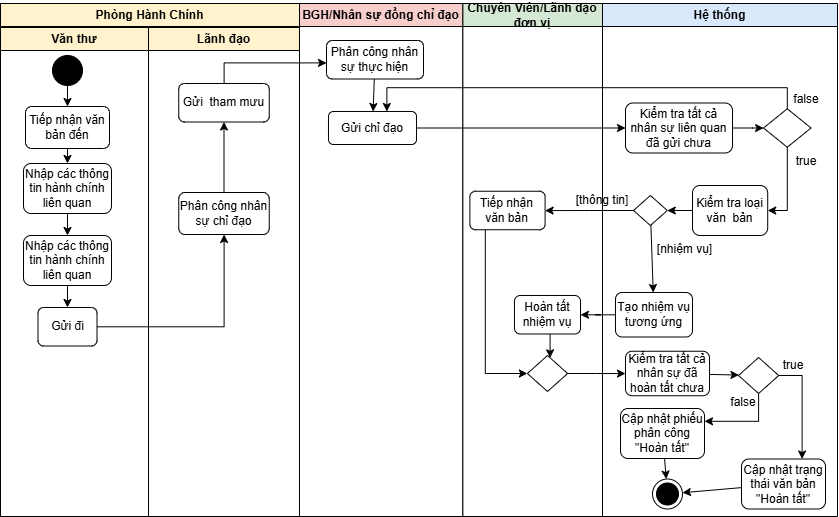
\includegraphics[width=\linewidth]{image/uml/doc_activity.png}
    \caption{Sơ đồ hoạt động quy trình xử lý văn bản đến}
    \label{fig:DOC_AC}
\end{figure}

Sơ đồ hoạt động Hình~\ref{fig:DOC_AC} mô tả chi tiết chu trình luân chuyển và xử lý văn bản đến xuyên suốt qua 4 phân vùng trách nhiệm: Văn thư Trường, Lãnh đạo Phòng Hành chính -- Tổng hợp, Ban Giám hiệu và các Đơn vị/Cá nhân thụ lý. Quy trình khởi đầu từ khi Văn thư tiếp nhận văn bản bên ngoài, hệ thống kích hoạt Quỹ số tự động cấp số đến duy nhất và sinh các bước quy trình mẫu. Sau khi hoàn tất cập nhật thông tin hành chính và tệp scan đính kèm, Lãnh đạo Phòng Hành chính nghiên cứu nội dung, ghi nhận ý kiến tham mưu đề xuất và lập dự thảo phân công trên Phiếu Giải Quyết để chuyển tiếp trình Ban Giám hiệu.

Tại phân vùng Ban Giám hiệu, hệ thống thiết lập khóa giao dịch cơ sở dữ liệu (\texttt{pg\_advisory\_xact\_lock}) nhằm loại trừ xung đột dữ liệu khi nhiều lãnh đạo cùng ra ý kiến chỉ đạo đồng thời. Văn bản chỉ được chuyển sang trạng thái Đã triển khai (\texttt{sentToDepartments}) khi có sự đồng thuận đầy đủ của Người chỉ đạo chính và tất cả Người đồng chỉ đạo. Ngay tại thời điểm triển khai, phân hệ tự động kích hoạt tạo cây Nhiệm vụ (Mission/Task) liên phòng ban và gửi thông báo thời gian thực đến các đơn vị thụ lý. Khi tiếp nhận văn bản, cán bộ đơn vị được tự động thêm vào nhiệm vụ liên kết; các văn bản thuần thông tin hoặc nhận để biết sẽ được tự động hoàn tất ngay khi bấm tiếp nhận. Đối với các văn bản giao nhiệm vụ, đơn vị triển khai thực hiện công việc chuyên môn hoặc khởi tạo dự thảo Văn bản đi phúc đáp liên kết, sau đó báo cáo hoàn thành trên Phiếu Giải Quyết. Khi 100\% các đơn vị thực hiện chính và phối hợp đều đã hoàn thành phần việc được giao, hệ thống tự động nâng trạng thái văn bản lên Hoàn thành (\texttt{departmentsDone}), khép lại toàn bộ vòng đời xử lý văn bản một cách chặt chẽ và minh bạch.
